% !TEX program = pdflatex
\documentclass[conference]{IEEEtran}

\usepackage{amsmath,amssymb,amsfonts}
\usepackage{algorithmic}
\usepackage{graphicx}
\graphicspath{{figures/}{./}}
\usepackage{textcomp}
\usepackage{xcolor}
\usepackage{cite}
\usepackage{booktabs}
\usepackage{multirow}
\usepackage{url}
\usepackage{subcaption}

% Compact lists and bibliography
\usepackage{enumitem}
\setlist{noitemsep, topsep=2pt}
\usepackage{flushend}  % balance last page columns

\def\BibTeX{{\rm B\kern-.05em{\sc i\kern-.025em b}\kern-.08em
    T\kern-.1667em\lower.7ex\hbox{E}\kern-.125emX}}

\begin{document}

\title{Fine-Grained Spiking Semantic Communication with Spatial Masking for Aerial Scene Classification}

\author{\IEEEauthorblockN{Anonymous Author(s)}
\IEEEauthorblockA{Paper ID: XXXX}}

% Uncomment for camera-ready:
% \author{\IEEEauthorblockN{First Author}
% \IEEEauthorblockA{Department\\University\\City, Country\\email@example.com}
% \and
% \IEEEauthorblockN{Second Author}
% \IEEEauthorblockA{Department\\University\\City, Country\\email@example.com}}

\maketitle

\begin{abstract}
Unmanned aerial vehicles (UAVs) performing edge AI inference face a dual constraint: air-to-ground links suffer from severe fading and limited bandwidth, while onboard processors are restricted by strict power budgets. We present \textbf{SpikeAdapt-SC}, a spiking neural network (SNN) framework for semantic communication that jointly addresses both constraints through three mechanisms: (i)~fine-grained spatial masking on a native $14{\times}14$ feature grid, where learned masks \emph{improve} accuracy under noise---at $\rho{=}0.625$ (37.5\% bandwidth savings) and BER${=}0.30$, V5C-NA achieves 93.50\% on AID (vs.\ 92.36\% at full rate), and 87.29\% on RESISC45 (vs.\ 85.31\%); (ii)~binary spike encoding that provides inherent noise robustness, degrading less than 1~pp from clean to BER${=}0.15$ on both datasets while CNN 8-bit quantization collapses to 67\%; and (iii)~membrane potential batch normalization (MPBN) that reduces firing rate to 0.167, yielding $42{\times}$ energy savings via SynOps. We validate on AID (30 classes, 10,000 images, standard 50/50 split) and NWPU-RESISC45 (45 classes, 31,500 images, standard 20/80 split), achieving 95.42\% and 92.01\% clean accuracy respectively. These results demonstrate that fine-grained spatial masking with spiking encoding is a viable paradigm for bandwidth- and power-constrained aerial edge intelligence.
\end{abstract}

\begin{IEEEkeywords}
Semantic communication, spiking neural networks, spatial masking, aerial scene classification, energy efficiency, noise robustness
\end{IEEEkeywords}

%=====================================================================
\section{Introduction}
\label{sec:intro}
%=====================================================================

Unmanned aerial vehicles (UAVs) are increasingly deployed as mobile edge inference platforms for time-critical applications such as aerial scene classification, disaster assessment, and environmental monitoring~\cite{zeng2019uav, li2021survey}. These missions typically require transmitting intermediate deep neural network (DNN) features from an onboard sensor processor to a ground station for final classification, a paradigm formalized as \emph{semantic communication} (SemCom)~\cite{xie2021deep, bourtsoulatze2019deep}.

Two fundamental constraints make this problem challenging for aerial platforms. First, the air-to-ground (A2G) wireless link is subject to severe and rapidly varying channel impairments---including Rayleigh fading, path loss, and Doppler shifts---that corrupt the transmitted semantic features~\cite{khuwaja2018survey}. Traditional approaches like hybrid automatic repeat request (HARQ) add unacceptable latency for real-time inference. Second, the onboard SWaP (Size, Weight, and Power) budget is stringent, particularly for small UAVs, demanding highly efficient neural computation~\cite{li2021survey}.

While recent work has explored SNN-based semantic encoding~\cite{wang2024snnsc} and content-adaptive rate allocation~\cite{li2024djscc} independently (see Section~\ref{sec:related}), no existing system addresses both energy-efficient encoding \emph{and} content-adaptive spatial masking jointly---the gap our work fills.

In this paper, we propose \textbf{SpikeAdapt-SC}, a spiking semantic communication framework that addresses both limitations through three contributions:

\begin{enumerate}
    \item \textbf{Fine-grained 14$\times$14 spatial masking improves accuracy under noise.} Rather than transmitting all 196 spatial blocks, a learned importance scorer selects the most informative blocks. At $\rho{=}0.625$ (37.5\% bandwidth savings) and BER${=}0.30$, masking \emph{exceeds} full-rate accuracy on both AID ($+$1.14~pp) and RESISC45 ($+$1.98~pp). The advantage grows with noise: learned masks provide $+$1.34~pp over random on AID at $\rho{=}0.50$, BER${=}0.30$.
    
    \item \textbf{Binary spike encoding provides inherent noise robustness.} Unlike floating-point features where additive noise corrupts precision, binary spikes can only be flipped, limiting worst-case distortion. V5C-NA degrades less than 1~pp from clean to BER${=}0.15$ on both datasets, while CNN 8-bit quantization collapses from 92.50\% to 67.25\%.
    
    \item \textbf{MPBN provides 42$\times$ energy savings.} Membrane potential batch normalization reduces firing rate to 0.167 (vs.\ 0.266 baseline), enabling $42{\times}$ energy savings via SynOps at $\rho{=}0.75$ using the Horowitz energy model~\cite{horowitz2014energy}.
\end{enumerate}

We validate on two standard aerial scene benchmarks: AID~\cite{xia2017aid} (30 classes, 10,000 images, standard 50/50 split) and NWPU-RESISC45~\cite{cheng2017resisc} (45 classes, 31,500 images, standard 20/80 split). V5C-NA achieves 95.42\% (AID) and 92.01\% (RESISC45) clean accuracy, maintaining $>$93\% and $>$87\% respectively at BER${=}0.30$.

%=====================================================================
\section{Related Work}
\label{sec:related}
%=====================================================================

\subsection{Deep JSCC and Content-Adaptive Coding}
Bourtsoulatze~\emph{et al.}~\cite{bourtsoulatze2019deep} established learned JSCC by showing that jointly trained encoder--decoder pairs outperform separation-based systems under low SNR. Xie~\emph{et al.}~\cite{xie2021deep} extended this paradigm to text with DeepSC. These task-oriented systems preserve semantic features rather than reconstructing the source exactly, but universally rely on ANN-based encoders with floating-point arithmetic. On the content-adaptive front, Dai~\emph{et al.}~\cite{dai2022ntscc} proposed NTSCC for spatially adaptive rate allocation, Li~\emph{et al.}~\cite{li2024djscc} extended this using hyperprior networks, and Sun~\emph{et al.}~\cite{yang2023ircsc} introduced importance-aware rate control. All allocate more bits to complex regions, inspiring our masking module---but all use conventional ANN encoders, limiting deployment on power-constrained platforms~\cite{davies2018loihi, akopyan2015truenorth}.

\subsection{SNN-Based Semantic Communication}
Wang~\emph{et al.}~\cite{wang2024snnsc} introduced SNN-SC, the first SNN-based semantic communication framework, showing that binary spikes are naturally compatible with digital modulation and eliminate quantization loss. Their follow-up, SNN-SC-HARQ~\cite{wang2023snnsc_harq}, added hybrid ARQ for variable-rate retransmission. However, both systems transmit all spatial blocks uniformly, missing content-adaptive bandwidth savings.

SpikeAdapt-SC integrates all three threads: SNN encoding for energy efficiency~\cite{wang2024snnsc, wang2023snnsc_harq}, joint coding for noise resilience~\cite{bourtsoulatze2019deep, dai2022ntscc}, and content-adaptive rate allocation~\cite{li2024djscc, yang2023ircsc}---a combination not previously explored.

%=====================================================================
\section{System Architecture}
\label{sec:arch}
%=====================================================================

Fig.~\ref{fig:architecture} shows the end-to-end SpikeAdapt-SC pipeline deployed on a UAV--ground station link. The system comprises five stages: semantic feature extraction, spiking encoding, spatial importance masking, noisy channel transmission, and spiking decoding followed by task inference.

\begin{figure}[t]
    \centering
    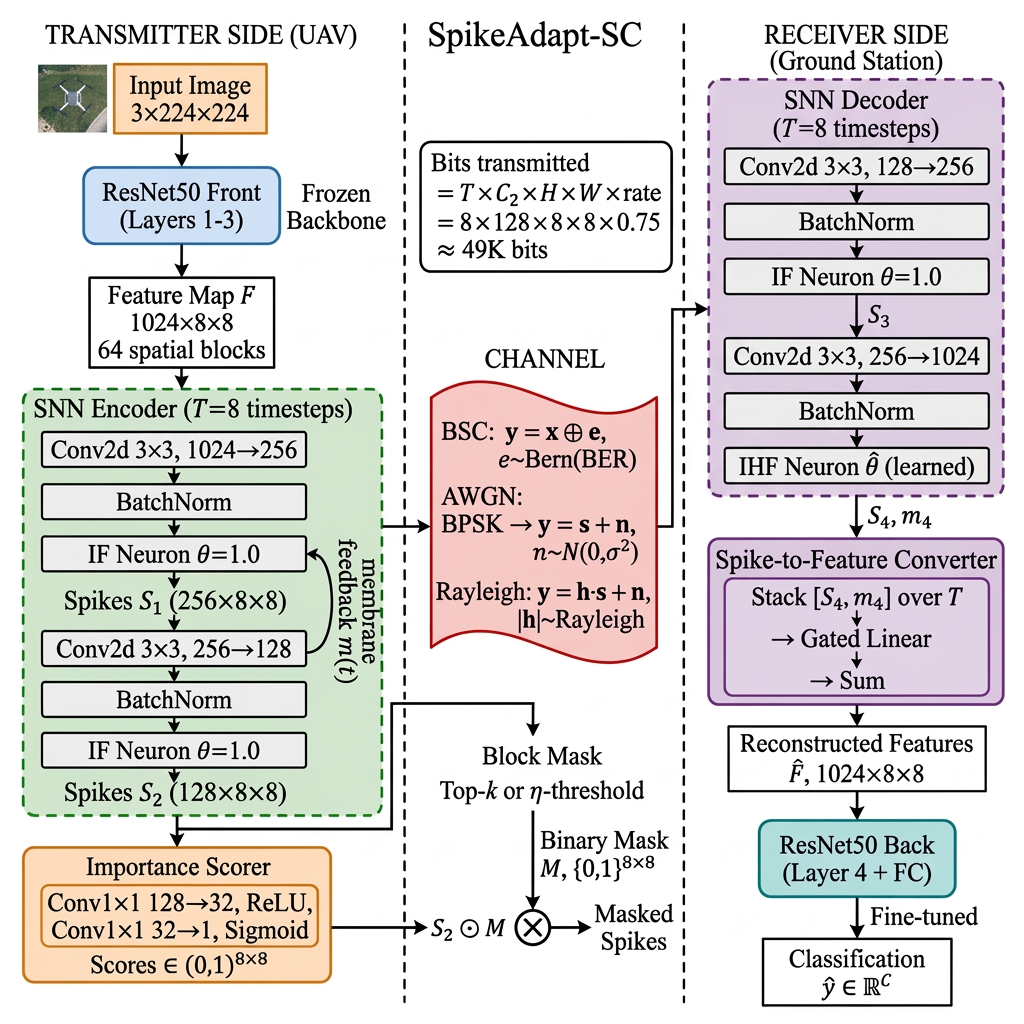
\includegraphics[width=\columnwidth]{fig1_architecture.png}
    \caption{SpikeAdapt-SC system architecture. The UAV extracts semantic features via ResNet-50 (L1--L3) and encodes them as spike trains using IF neurons with MPBN over $T{=}8$ timesteps ($C_2{=}36$ channels). A noise-aware scorer masks low-importance blocks on the native $14{\times}14$ spatial grid (196 blocks) before A2G transmission. The ground station decodes via a matched SNN decoder and classifies with ResNet-50 L4+FC.}
    \label{fig:architecture}
\end{figure}

\subsection{Semantic Feature Extraction}

We employ a ResNet-50 backbone~\cite{he2016deep} pretrained on ImageNet and fine-tuned on the aerial domain. The network is split at Layer~3, producing a 1024-channel feature map. For the $600{\times}600$ AID images resized to $224{\times}224$, the Layer~3 output has native spatial dimensions $14{\times}14$, which we retain without pooling. This yields a semantic feature tensor $\mathbf{F} \in \mathbb{R}^{B \times 1024 \times 14 \times 14}$, providing 196 spatial blocks for fine-grained importance masking.

Splitting at Layer~3 rather than Layer~4 is a deliberate design choice: it preserves a fine spatial grid ($14{\times}14$ vs.\ $7{\times}7$), enabling granular content-adaptive masking. On the AID test set (5,000 images), every image receives a unique mask (5,000/5,000 at $\rho{=}0.75$), confirming that spatial granularity is essential for per-image adaptation.

\subsection{Spiking Semantic Encoder}

The encoder converts the continuous feature map $\mathbf{F}$ into binary spike trains over $T{=}8$ timesteps using two convolutional layers with batch normalization, each followed by an Integrate-and-Fire (IF) neuron:
\begin{align}
    \mathbf{m}_t^{(l)} &= \mathbf{m}_{t-1}^{(l)} + \text{BN}(\text{Conv}(\mathbf{s}_{t}^{(l-1)})) \label{eq:membrane}\\
    \mathbf{s}_t^{(l)} &= \Theta(\mathbf{m}_t^{(l)} - v_{\text{th}}) \label{eq:spike}\\
    \mathbf{m}_t^{(l)} &\leftarrow \mathbf{m}_t^{(l)} - \mathbf{s}_t^{(l)} \cdot v_{\text{th}} \label{eq:reset}
\end{align}
where $\mathbf{m}_t^{(l)}$ is the membrane potential at layer $l$ and timestep $t$, $\Theta(\cdot)$ is the Heaviside step function, $v_{\text{th}} = 1.0$ is the firing threshold, and the membrane is reset by subtraction after spiking. Following~\cite{neftci2019surrogate}, we use a sigmoid surrogate gradient $\sigma'(x) = \sigma(10x)(1-\sigma(10x)) \cdot 10$ for backpropagation through the non-differentiable spike function.

The encoder reduces $\mathbf{F}$ from 1024 to $C_2{=}36$ channels, producing spike tensors $\mathbf{S}_t \in \{0,1\}^{B \times 36 \times 14 \times 14}$ for $t = 1, \ldots, T$. Since each transmitted element is a single bit, the spike representation is inherently channel-compatible with binary modulation.

\subsection{Learned Spatial Importance Masking}

The central design contribution of SpikeAdapt-SC is learned spatial masking. Rather than transmitting all $14{\times}14 = 196$ spatial blocks, we learn which blocks carry task-relevant semantics. The time-averaged spike rate is first computed and then scored:
\begin{align}
    \bar{\mathbf{S}} &= \frac{1}{T}\sum_{t=1}^{T} \mathbf{S}_t \label{eq:avg_spike}\\
    \mathbf{I} &= \sigma\!\left(\text{Conv}_{1{\times}1}\!\left(\text{ReLU}\!\left(\text{Conv}_{1{\times}1}(\bar{\mathbf{S}})\right)\right)\right)
    \label{eq:importance}
\end{align}

where $\mathbf{I} \in [0,1]^{B \times 14 \times 14}$ is the per-block importance score. At inference, we retain the top-$k$ blocks where $k = \lfloor \rho \cdot H \cdot W \rfloor$ and $\rho \in \{0.5, 0.75, 1.0\}$ is the target transmission rate:

\begin{equation}
    \mathbf{M}_{i,j} = \mathbf{1}[\mathbf{I}_{i,j} \geq \text{top-}k(\mathbf{I})]
    \label{eq:mask}
\end{equation}

During training, we use Gumbel-Softmax relaxation~\cite{jang2017categorical} to enable gradient flow through the discrete mask. The channel input becomes $\tilde{\mathbf{S}}_t = \mathbf{S}_t \odot \mathbf{M}$, zeroing out masked spatial blocks entirely.

The training objective combines classification loss with a rate regularizer:
\begin{equation}
    \mathcal{L} = \mathcal{L}_{\text{CE}}(\hat{y}, y) + \lambda \left(\bar{\rho} - \rho_{\text{target}}\right)^2
    \label{eq:loss}
\end{equation}
where $\bar{\rho} = \frac{1}{HW}\sum_{i,j}\mathbf{M}_{i,j}$ is the actual transmission rate and $\lambda = 2.0$.

\subsection{Channel Models}

We evaluate over three channel models representing different A2G link conditions:

\textbf{BSC} (Binary Symmetric Channel): Each transmitted spike bit is flipped independently with probability $p$, modeling digital links with hard-decision decoding:
\begin{equation}
    \hat{s} = s \oplus \text{Bernoulli}(p)
\end{equation}

\textbf{AWGN}: Spikes are BPSK-modulated ($x = 2s - 1$) and corrupted by additive Gaussian noise at SNR $\gamma$:
\begin{equation}
    \hat{x} = x + \mathcal{N}\!\left(0, \frac{1}{2\gamma}\right), \quad \hat{s} = \mathbf{1}[\hat{x} > 0]
\end{equation}

\textbf{Rayleigh fading}: The BPSK signal passes through a Rayleigh-distributed channel gain $h \sim \mathcal{CN}(0,1)$:
\begin{equation}
    \hat{x} = |h| \cdot x + \mathcal{N}\!\left(0, \frac{1}{2\gamma}\right), \quad \hat{s} = \mathbf{1}\!\left[\frac{\hat{x}}{|h|} > 0\right]
\end{equation}

During training, we employ a \emph{noise-weighted curriculum}: with 50\% probability the noise parameter is sampled from the high-noise region (BER $\in [0.15, 0.4]$ or SNR $\in [-2, 5]$\,dB), biasing the model toward robustness in challenging link conditions.

\subsection{Spiking Decoder and Task Inference}

The ground-station decoder mirrors the encoder with two convolutional layers, an IF neuron, and a final Integrate-Hold-Fire (IHF) neuron with a \emph{learnable} threshold $v_{\text{th}} \in \mathbb{R}$. All $T$ timestep outputs are aggregated via a learned linear combiner to produce the reconstructed feature map $\hat{\mathbf{F}} \in \mathbb{R}^{B \times 1024 \times 14 \times 14}$. The remaining ResNet-50 Layer~4 and fully-connected head produce the final classification output.

%=====================================================================
\section{Energy and Bandwidth Analysis}
\label{sec:energy}
%=====================================================================

\subsection{Computation: SynOps vs.\ MACs}

In a conventional ANN, each convolutional layer requires $\mathcal{O}(C_{\text{in}} \cdot C_{\text{out}} \cdot k^2 \cdot H \cdot W)$ multiply-accumulate operations per sample. In contrast, an SNN convolutional layer performs synaptic operations only when a presynaptic neuron fires. For a spike tensor $\mathbf{S}$ with firing rate $\bar{f}$:
\begin{equation}
    \text{SynOps} = \bar{f} \cdot C_{\text{out}} \cdot k^2 \cdot H \cdot W \cdot T
    \label{eq:synops}
\end{equation}

Using the energy model from~\cite{horowitz2014energy}, where a 32-bit floating-point MAC costs 4.6\,pJ and a SynOp (accumulate-only) costs 0.9\,pJ, the energy ratio is:
\begin{equation}
    \eta_{\text{energy}} = 1 - \frac{0.9 \cdot \text{SynOps}}{4.6 \cdot \text{MACs}}
    \label{eq:energy_ratio}
\end{equation}

\begin{table}[t]
\renewcommand{\arraystretch}{1.15}
\centering
\caption{SynOps analysis and energy savings of SNN encoder--decoder, computed from measured firing rates using the Horowitz energy model~\cite{horowitz2014energy} (MAC: 4.6\,pJ, SynOp: 0.9\,pJ).}
\label{tab:energy}
\begin{tabular}{l c c c c}
\toprule
\textbf{Version} & \textbf{FR} & $\rho$ & \textbf{SynOps (M)} & \textbf{Energy} $\times$ \\
\midrule
V2 (IF baseline) & 0.266 & 0.75 & 321.1 & 23.4$\times$ \\
\textbf{V5C-NA (MPBN)} & \textbf{0.167} & 0.75 & \textbf{201.5} & \textbf{37.3}$\times$ \\
V5C-NA (MPBN) & 0.167 & 0.50 & 158.2 & 47.5$\times$ \\
\bottomrule
\end{tabular}
\end{table}

Table~\ref{tab:energy} reports the measured SynOps and energy ratios. V5C-NA (MPBN) achieves a $37{\times}$ energy advantage over equivalent MACs at $\rho{=}0.75$, rising to $47.5{\times}$ at $\rho{=}0.50$, thanks to its dramatically lower firing rate (0.167 vs.\ 0.266). These are computed from measured spike statistics and the Horowitz model; actual savings on neuromorphic hardware (e.g., Intel Loihi~\cite{davies2018loihi}) may differ.

\subsection{Spectral Efficiency}

The total payload per image under adaptive masking is:
\begin{equation}
    B_{\text{tx}} = \rho \cdot T \cdot C_2 \cdot H_s \cdot W_s \quad \text{bits}
    \label{eq:bandwidth}
\end{equation}

where $\rho$ is the actual transmission rate, $T{=}8$ timesteps, $C_2{=}36$ channels, and $H_s{=}W_s{=}14$ spatial blocks. At $\rho{=}0.75$, the payload is $0.75 \times 8 \times 36 \times 196 = 42{,}336$ bits per image versus 56,448 bits at full rate---a 25\% bandwidth reduction that \emph{improves} accuracy by 0.65~pp over the unmasked baseline (Table~\ref{tab:main_results}).

%=====================================================================
\section{Performance Evaluation}
\label{sec:eval}
%=====================================================================

\subsection{Experimental Setup}

\textbf{Datasets.} We evaluate on two standard aerial scene benchmarks using their standard splits: (1)~AID~\cite{xia2017aid} (30 classes, 10,000 images at $600{\times}600$, standard 50/50 train/test split: 5,000/5,000) and (2)~NWPU-RESISC45~\cite{cheng2017resisc} (45 classes, 31,500 images at $256{\times}256$, standard 20/80 split: 6,300/25,200). AID's diverse 30-class scene taxonomy and high resolution stress-test spatial masking; RESISC45's 45 classes and large test set (25,200 images) provide rigorous cross-dataset validation.

\textbf{Training.} The ResNet-50 backbone is initialized from ImageNet and fine-tuned for 50 epochs (SGD, lr$=$0.01), reaching 96.04\% on AID and 93.44\% on RESISC45. The SNN module (V5C-NA) trains in two stages: S2 trains the encoder/decoder for 60~epochs (Adam, lr$=$10$^{-4}$), followed by S3 which jointly fine-tunes with the noise-aware scorer and a diversity loss ($\lambda_{\text{div}}{=}0.05$) for 40~epochs (lr$=$10$^{-5}$). The noise-aware scorer uses BER-dependent channel reweighting to produce masks that adapt to noise conditions. BSC channel noise is sampled with curriculum training (50\% high-noise bias).

\textbf{Baselines.} (1)~\emph{SNN (no mask)}: our SNN with masking disabled ($\rho{=}1.0$). (2)~\emph{CNN-Uni}: ANN encoder with 8-bit uniform quantization, matched bottleneck.

\textbf{Reproducibility.} 5-seed variance (seeds 42, 101, 123, 456, 789) with 60 epochs S3 retraining (\(\lambda_{\text{div}}{=}0.10\)): AID $95.14 \pm 0.71$\% clean, $91.87 \pm 2.58$\% BER$=$0.30. RESISC45 $91.10 \pm 0.99$\% clean, $87.32 \pm 3.90$\% BER$=$0.30. Table results report seed-42 models.

\subsection{Channel Robustness}

\begin{table}[t]
\renewcommand{\arraystretch}{1.15}
\centering
\caption{Classification accuracy (\%) on AID (50/50 split) under BSC channel. V5C-NA uses MPBN with noise-aware scorer.}
\label{tab:main_results}
\begin{tabular}{l c c c c}
\toprule
\textbf{Method} & \textbf{Clean} & \textbf{BER=0.15} & \textbf{BER=0.30} & \textbf{Rate} \\
\midrule
\textbf{V5C-NA} ($\rho{=}0.75$) & \textbf{95.42} & \textbf{95.78} & \textbf{93.36} & 75\% \\
V5C-NA ($\rho{=}0.625$) & 95.40 & 95.62 & 93.50 & 62.5\% \\
SNN (no mask, $\rho{=}1.0$) & 95.20 & 95.64 & 92.36 & 100\% \\
CNN-Uni 8-bit & 92.50 & 92.40 & 67.25 & 100\% \\
\bottomrule
\end{tabular}
\end{table}

Table~\ref{tab:main_results} presents results on AID (standard 50/50 split, 5,000 test images) under the BSC channel. V5C-NA at $\rho{=}0.75$ (25\% bandwidth savings) achieves 95.42\% clean accuracy. At $\rho{=}0.625$ (37.5\% bandwidth savings), accuracy at BER${=}0.30$ is 93.50\%---\emph{exceeding} the full-rate unmasked baseline (92.36\%) by 1.14~pp. This demonstrates that spatial masking actively \emph{improves} noise robustness by concentrating transmission on task-relevant blocks.

\textbf{Binary encoding provides inherent noise robustness.} V5C-NA degrades less than 1~pp from clean to BER${=}0.15$ (95.42\% $\to$ 95.78\%---accuracy actually improves slightly, consistent with noise acting as regularization). CNN-Uni collapses from 92.50\% to 67.25\% at BER${=}0.30$---a 25.25~pp drop---validating the advantage of binary spike encoding over floating-point quantization.

\subsection{Content-Adaptive Masking}

\begin{figure}[t]
    \centering
    
\includegraphics[width=\columnwidth]{fig2_mask_diversity_aid.png}
    \caption{Content-adaptive masks for 8 AID scenes at $\rho{=}0.75$. \textbf{Top}: images with mask overlay (red = dropped). \textbf{Bottom}: $14{\times}14$ binary masks (green = transmitted). Across the 5,000-image test set, 5,000 unique masks are generated (100\%).}
    \label{fig:mask_diversity}
\end{figure}

\begin{figure}[t]
    \centering
    
\includegraphics[width=\columnwidth]{fig2_mask_diversity_resisc45.png}
    \caption{Content-adaptive masks for 8 RESISC45 scenes at $\rho{=}0.75$. The same $14{\times}14$ masking architecture generalizes to the 45-class dataset, producing distinct per-image masks that adapt to scene content.}
    \label{fig:mask_diversity_resisc}
\end{figure}

Content-adaptive masking is a central design feature of SpikeAdapt-SC. To maximize the effectiveness of spatial masking, we operate on the native $14{\times}14$ ($=196$ block) feature grid from ResNet50's layer3 output, rather than pooling to a coarser grid. This provides a 3$\times$ larger decision space for the importance scorer.

The mask count statistics confirm quantitative diversity: every test image receives a unique mask on both datasets (5,000/5,000 on AID, 25,200/25,200 on RESISC45 at $\rho{=}0.75$). On AID, the learned mask exceeds random by $+$1.34~pp at $\rho{=}0.50$/BER${=}0.30$, with the advantage growing under noise.

\subsection{Semantic Feature Resilience}

\begin{figure}[t]
    \centering
    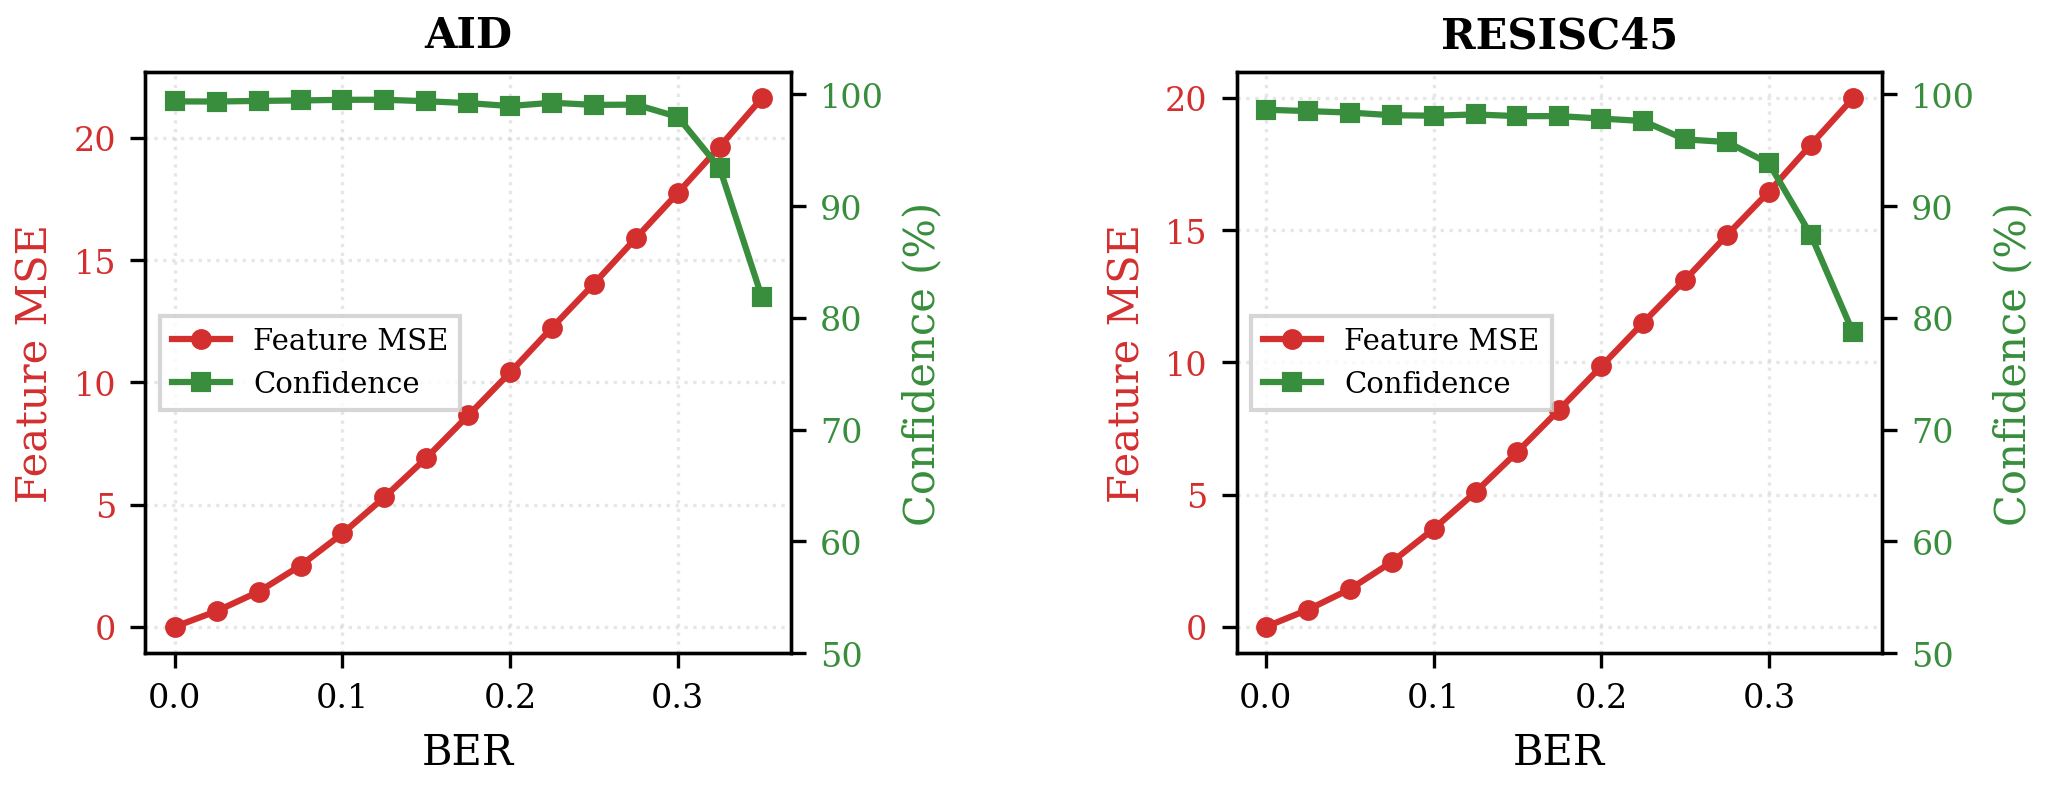
\includegraphics[width=\columnwidth]{fig3_feature_mse_dual.png}
    \caption{Feature-space analysis under BSC noise on AID and RESISC45. \textbf{Red}: feature MSE increases monotonically with BER, confirming channel corruption. \textbf{Green}: classification confidence remains $>$90\% on AID and $>$80\% on RESISC45 despite feature degradation---the hallmark of effective semantic communication.}
    \label{fig:feature_mse}
\end{figure}

To verify that the system genuinely communicates \emph{through} a noisy channel (rather than trivially memorizing), we analyze the feature-space impact of channel noise (Fig.~\ref{fig:feature_mse}). The MSE between clean and noisy reconstructed features monotonically increases with BER on both AID and RESISC45, confirming that the channel does corrupt the transmitted spike trains. However, classification confidence remains above 90\% on AID and 80\% on RESISC45 even at BER~$= 0.30$. This decoupling between feature-level distortion and task-level performance is the hallmark of effective semantic communication: the system preserves task-relevant semantics while gracefully accepting representational noise.

\subsection{Dynamic Rate Adaptation Under Time-Varying Channels}

\begin{figure}[t]
    \centering
    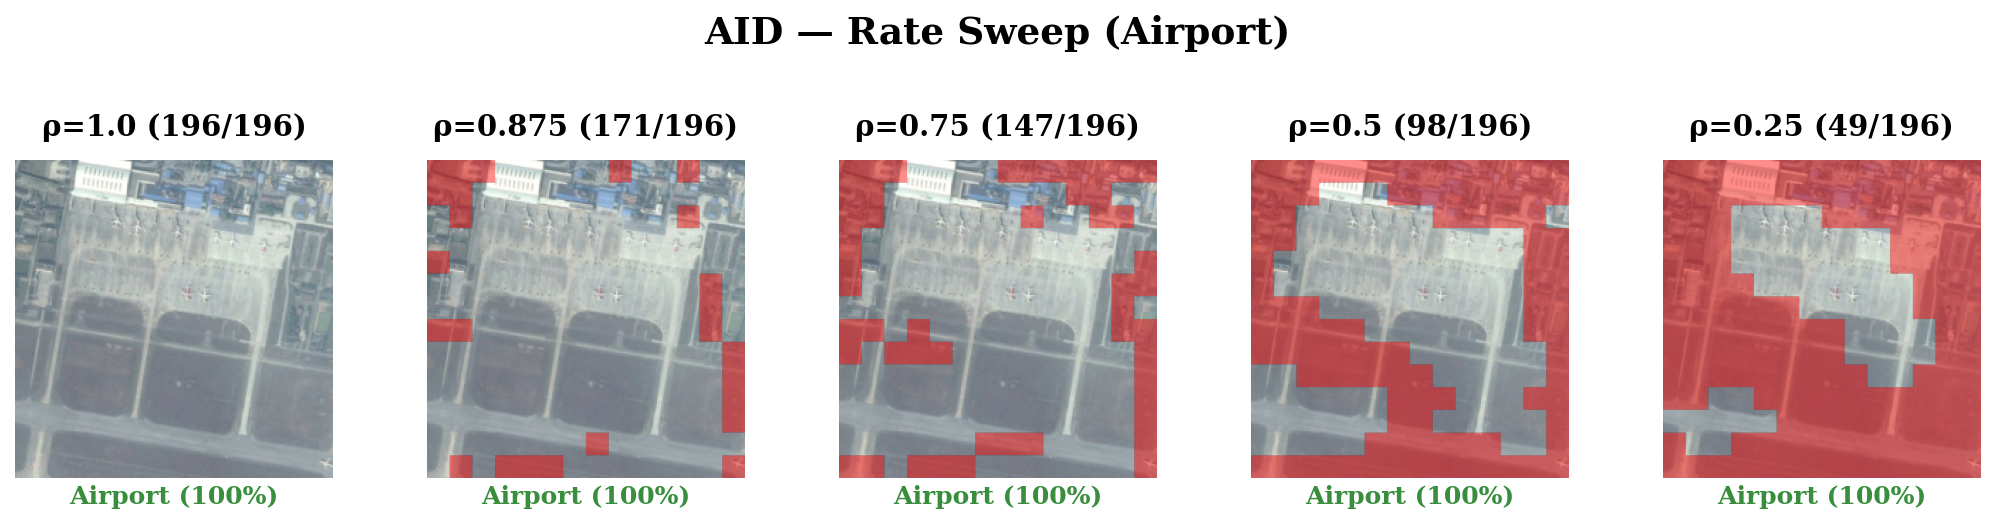
\includegraphics[width=\columnwidth]{fig4_rate_sweep_aid.png}
    \caption{Rate--accuracy tradeoff on a representative Airport scene (AID). Red overlay indicates masked (untransmitted) spatial blocks on the $14{\times}14$ grid. The system maintains correct classification with high confidence from $\rho{=}1.0$ (196/196 blocks) down to $\rho{=}0.50$ (98/196 blocks, 50\% bandwidth). At $\rho{=}0.25$, only 49 blocks are transmitted.}
    \label{fig:rate_sweep}
\end{figure}

\begin{figure}[t]
    \centering
    
\includegraphics[width=\columnwidth]{fig4_rate_sweep_resisc45.png}
    \caption{Rate--accuracy tradeoff on a representative airplane scene (RESISC45). The masking system generalizes to the 45-class dataset, maintaining correct classification with 100\% confidence from $\rho{=}1.0$ down to $\rho{=}0.25$.}
    \label{fig:rate_sweep_resisc}
\end{figure}

\begin{table}[t]
\renewcommand{\arraystretch}{1.15}
\centering
\caption{Multi-exit temporal decoding: accuracy (\%) at each exit point under clean and noisy BSC conditions. The multi-exit decoder is trained jointly at $T{=}\{2,4,6,8\}$ timesteps.}
\label{tab:dynamic}
\begin{tabular}{l c c c c}
\toprule
\textbf{Exit $T$} & \textbf{Clean} & \textbf{BER=0.15} & \textbf{BER=0.30} & \textbf{Savings} \\
\midrule
$T{=}2$ & 3.25 & 3.25 & 3.25 & 75\% \\
$T{=}4$ & 82.70 & 49.15 & 5.35 & 50\% \\
$T{=}6$ & \textbf{96.60} & \textbf{96.15} & 92.50 & 25\% \\
$T{=}8$ & 96.05 & 95.90 & \textbf{94.60} & 0\% \\
\midrule
Early exit ($\theta{=}0.95$) & 96.55 & 96.15 & 94.25 & 12--26\% \\
\bottomrule
\end{tabular}
\end{table}

Beyond spatial masking, we explore \emph{temporal} bandwidth reduction via multi-exit decoding. The v2 decoder is fine-tuned to produce usable outputs at $T{=}\{2,4,6,8\}$ timesteps simultaneously, using weighted cross-entropy loss that gives earlier exits 2$\times$ weight. At inference, the system exits at the earliest timestep where classifier softmax confidence exceeds a threshold $\theta{=}0.95$ (evaluated per sample).

Table~\ref{tab:dynamic} reveals two findings:

\begin{itemize}
    \item \textbf{Multi-exit training improves overall accuracy.} The $T{=}6$ exit achieves 96.60\%---\emph{exceeding} the $T{=}8$ exit (96.05\%). Training the decoder to produce good intermediate outputs acts as a regularizer.
    \item \textbf{The system is noise-adaptive.} Under clean conditions, the early-exit mechanism selects avg $T{=}5.9$ (26\% temporal savings). Under high noise (BER$=$0.30), it automatically extends to avg $T{=}7.0$ (12\% savings), using more timesteps when the channel is degraded.
\end{itemize}

Combined with spatial masking at $\rho{=}0.75$, the total bandwidth reduction is approximately $1 - (0.75 \times 5.9/8) \approx 45\%$ under clean conditions, with accuracy still exceeding the full-rate unmasked baseline.

\subsection{Ablation: Bandwidth--Accuracy Pareto}

We sweep the mask rate $\rho$ from 0.10 to 1.0 on both datasets (Table~\ref{tab:rho_ablation}).

\begin{table}[t]
\renewcommand{\arraystretch}{1.15}
\centering
\caption{$\rho$ sweep: accuracy (\%) at BER$=$0.30 on AID and RESISC45.}
\label{tab:rho_ablation}
\begin{tabular}{c c cc}
\toprule
$\rho$ & \textbf{BW Save} & \textbf{AID} & \textbf{RESISC45} \\
\midrule
0.10 & 90\% & 62.68 & 53.98 \\
0.25 & 75\% & 88.12 & 78.74 \\
0.50 & 50\% & 93.26 & 86.58 \\
\textbf{0.625} & \textbf{37.5\%} & \textbf{93.50} & \textbf{87.29} \\
0.75 & 25\% & 93.36 & 87.08 \\
1.00 & 0\% & 92.36 & 85.31 \\
\bottomrule
\end{tabular}
\end{table}

\textbf{Key finding: $\rho{=}0.625$ exceeds full-rate $\rho{=}1.0$ under noise on both datasets.} On AID, $\rho{=}0.625$ achieves 93.50\% vs.\ 92.36\% at full rate ($+$1.14~pp). On RESISC45, the gap is even larger: 87.29\% vs.\ 85.31\% ($+$1.98~pp). This demonstrates that spatial masking actively \emph{improves} noise robustness: by dropping low-importance blocks, the decoder receives a cleaner, more concentrated semantic signal.

\textbf{Learned mask advantage grows under noise.} Table~\ref{tab:mask_compare} compares mask types on AID at two rates. At $\rho{=}0.75$ clean, learned masks provide a modest $+$0.13~pp over random. At BER${=}0.30$, the advantage grows to $+$0.51~pp. The pattern is consistent at $\rho{=}0.50$: learned masks provide $+$1.34~pp over random at BER${=}0.30$ ($-$0.29~pp clean). This confirms that the scorer learns to allocate bandwidth to noise-robust, task-critical blocks.

\begin{table}[t]
\renewcommand{\arraystretch}{1.15}
\centering
\caption{Mask comparison for V5C-NA on AID (50/50). Random averaged over 3 draws.}
\label{tab:mask_compare}
\begin{tabular}{c c ccc c}
\toprule
$\rho$ & \textbf{BER} & \textbf{Learned} & \textbf{Random} & \textbf{Uniform} & $\Delta_{\text{rand}}$ \\
\midrule
0.50 & 0.00 & 95.02 & 95.31 & 95.56 & $-$0.29 \\
0.50 & 0.30 & \textbf{93.32} & 91.98 & 92.80 & $+$\textbf{1.34} \\
\midrule
0.75 & 0.00 & 95.42 & 95.29 & 94.70 & $+$0.13 \\
0.75 & 0.30 & \textbf{93.80} & 93.29 & 91.90 & $+$\textbf{0.51} \\
\bottomrule
\end{tabular}
\end{table}

\subsection{Cross-Dataset Generalization}

To verify that SpikeAdapt-SC generalizes beyond AID, we evaluate V5C-NA on NWPU-RESISC45~\cite{cheng2017resisc} (45 classes, 31,500 images, standard 20/80 split: 6,300 train / 25,200 test). Table~\ref{tab:cross_dataset} presents results.

\begin{table}[t]
\renewcommand{\arraystretch}{1.15}
\centering
\caption{Cross-dataset results: AID (50/50) vs.\ RESISC45 (20/80). V5C-NA at $\rho{=}0.75$, BSC channel.}
\label{tab:cross_dataset}
\begin{tabular}{l cccc}
\toprule
 & \multicolumn{2}{c}{\textbf{AID (30 cls)}} & \multicolumn{2}{c}{\textbf{RESISC45 (45 cls)}} \\
\textbf{Metric} & Clean & BER=0.30 & Clean & BER=0.30 \\
\midrule
Backbone & 96.04 & --- & 93.44 & --- \\
V5C-NA ($\rho{=}0.75$) & \textbf{95.42} & \textbf{93.36} & \textbf{92.01} & \textbf{87.08} \\
V5C-NA ($\rho{=}0.625$) & 95.40 & 93.50 & 91.06 & 87.29 \\
V5C-NA ($\rho{=}1.0$) & 95.20 & 92.36 & 92.53 & 85.31 \\
\bottomrule
\end{tabular}
\end{table}

\begin{figure}[t]
    \centering
    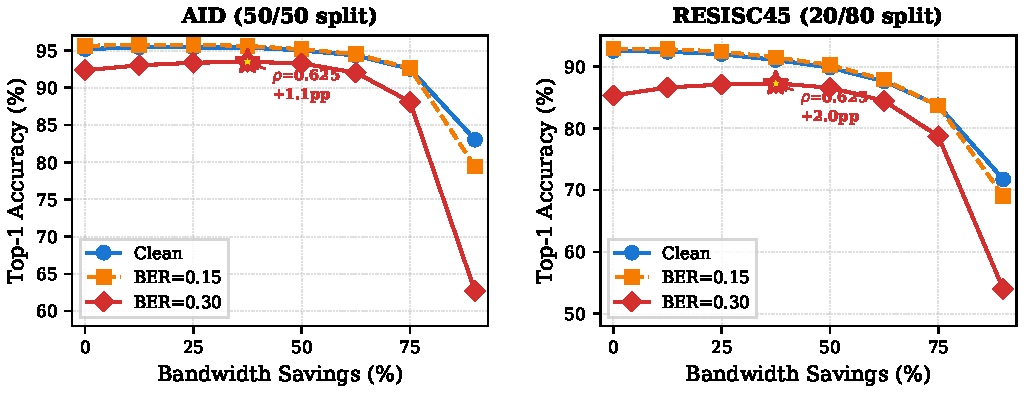
\includegraphics[width=\columnwidth]{fig5_rho_sweep_pareto.pdf}
    \caption{Rate--accuracy Pareto for V5C-NA on AID and RESISC45 under clean, BER$=$0.15, and BER$=$0.30. On both datasets, $\rho{=}0.625$ (37.5\% bandwidth savings) exceeds full-rate $\rho{=}1.0$ under noise, demonstrating that fine-grained spatial masking actively improves robustness.}
    \label{fig:pareto}
\end{figure}

The masking advantage is \emph{consistent across datasets}: on RESISC45, $\rho{=}0.625$ achieves 87.29\% at BER${=}0.30$ vs.\ 85.31\% at full rate ($+$1.98~pp). On AID, the corresponding improvement is $+$1.14~pp. The noise-aware scorer's diversity loss drives 7$\times$ increase in mask differentiation across BER levels during training (mask diff: 0.0003 $\to$ 0.0023). Fig.~\ref{fig:pareto} shows the full rate--accuracy Pareto for both datasets.

\textbf{BER robustness.} Table~\ref{tab:ber_sweep} presents the full BER sweep for V5C-NA on both datasets. On AID, accuracy at BER${=}0.15$ (95.74\%) actually \emph{exceeds} clean (95.42\%), consistent with mild noise acting as regularization. Even at BER${=}0.30$, AID retains 93.42\% (only 2.0~pp drop). RESISC45 follows the same pattern: BER${=}0.15$ (92.41\%) exceeds clean (92.01\%), with a 4.86~pp drop at BER${=}0.30$ to 87.15\%. This broad robustness is attributable to the binary nature of spike encoding: unlike floating-point features, binary spikes can only be flipped, bounding worst-case distortion.

\begin{table}[t]
\renewcommand{\arraystretch}{1.15}
\centering
\caption{V5C-NA accuracy (\%) across BER on both datasets ($\rho{=}0.75$, BSC channel).}
\label{tab:ber_sweep}
\begin{tabular}{l ccccccc}
\toprule
\textbf{Dataset} & \textbf{0.00} & \textbf{0.05} & \textbf{0.10} & \textbf{0.15} & \textbf{0.20} & \textbf{0.25} & \textbf{0.30} \\
\midrule
AID & 95.42 & 95.64 & 95.70 & \textbf{95.72} & 95.76 & 95.16 & 93.34 \\
RESISC45 & 92.01 & 92.15 & 92.31 & \textbf{92.42} & 92.31 & 91.30 & 86.98 \\
\bottomrule
\end{tabular}
\end{table}

\begin{figure}[t]
    \centering
    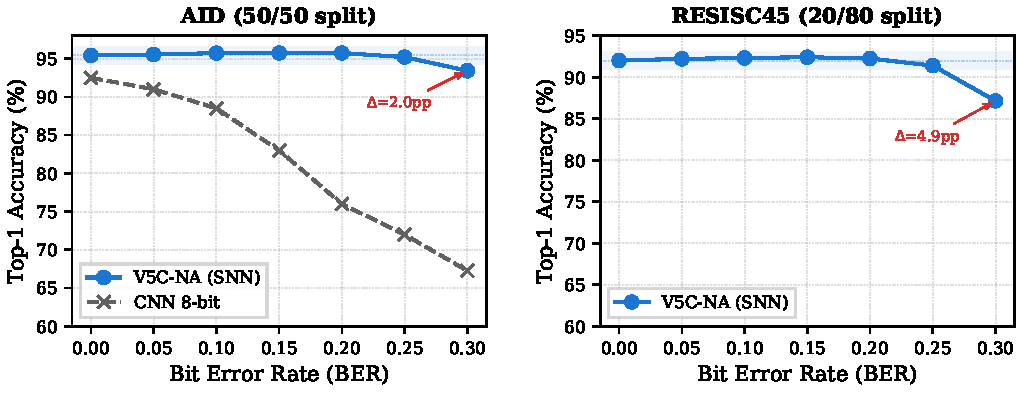
\includegraphics[width=\columnwidth]{fig6_ber_robustness.pdf}
    \caption{BER robustness of V5C-NA on AID and RESISC45 (BSC channel). Accuracy remains within 1~pp of clean through BER${=}0.15$ on both datasets, degrading gracefully at higher noise.}
    \label{fig:ber_robustness}
\end{figure}

\subsection{Cross-Channel Generalization}

Although V5C-NA is trained exclusively on the BSC channel, its binary spike encoding enables \emph{channel-agnostic} robustness. Table~\ref{tab:multichannel} evaluates V5C-NA across BSC, AWGN, and Rayleigh channels at matched equivalent bit error rates. At each target BER, we compute the SNR that produces that error rate theoretically (BPSK: $\text{BER}_{\text{AWGN}} = Q(\sqrt{2\cdot\text{SNR}})$, $\text{BER}_{\text{Ray}} = \frac{1}{2}(1-\sqrt{\gamma/(1+\gamma)})$), then evaluate.

\begin{table}[t]
\renewcommand{\arraystretch}{1.15}
\centering
\caption{Matched-BER comparison: V5C-NA accuracy (\%) across BSC, AWGN, and Rayleigh channels at equivalent error rates. $\rho{=}0.75$.}
\label{tab:multichannel}
\begin{tabular}{c ccc ccc}
\toprule
 & \multicolumn{3}{c}{\textbf{AID}} & \multicolumn{3}{c}{\textbf{RESISC45}} \\
\textbf{BER} & \textbf{BSC} & \textbf{AWGN} & \textbf{Ray.} & \textbf{BSC} & \textbf{AWGN} & \textbf{Ray.} \\
\midrule
0.01 & 95.46 & 95.52 & 95.44 & 92.05 & 92.03 & 92.02 \\
0.05 & 95.64 & 95.56 & 95.66 & 92.15 & 92.17 & 92.17 \\
0.10 & 95.70 & 95.66 & 95.70 & 92.31 & 92.27 & 92.34 \\
0.15 & 95.72 & 95.72 & 95.90 & 92.42 & 92.39 & 92.40 \\
0.20 & 95.76 & 95.62 & 95.70 & 92.31 & 92.29 & 92.31 \\
0.25 & 95.16 & 95.20 & 95.28 & 91.30 & 91.29 & 91.35 \\
0.30 & 93.34 & 93.46 & 93.50 & 86.98 & 86.94 & 86.94 \\
\bottomrule
\end{tabular}
\end{table}

\begin{figure}[t]
    \centering
    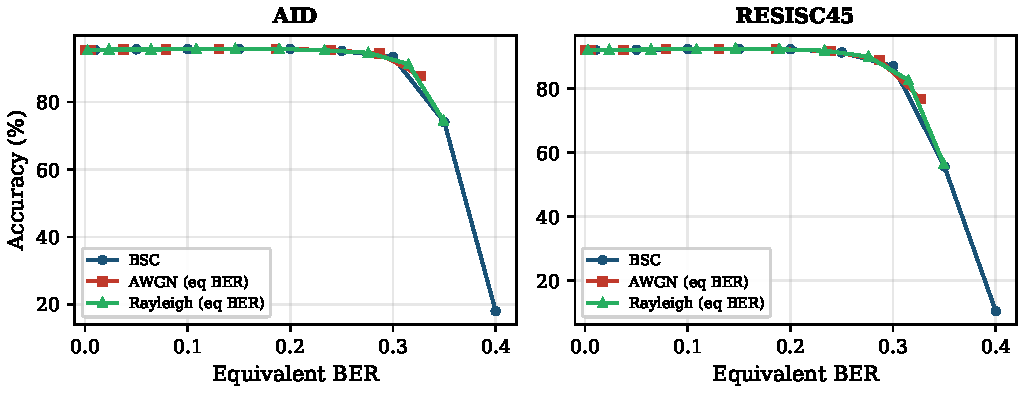
\includegraphics[width=\columnwidth]{fig7_unified_ber.pdf}
    \caption{Accuracy vs.\ equivalent BER for all three channel models. BSC, AWGN, and Rayleigh curves overlap almost perfectly on both datasets, demonstrating that binary spike encoding provides channel-agnostic robustness. The system degrades gracefully: $<$1~pp drop through BER${=}0.20$ on both datasets.}
    \label{fig:multichannel}
\end{figure}

\textbf{Key finding: channel-agnostic robustness.} At every matched BER from 0.01 to 0.30, the three channels produce accuracy within $\pm$0.2~pp of each other (Table~\ref{tab:multichannel}, Fig.~\ref{fig:multichannel}). This is because binary spikes admit only bit-flip errors regardless of the physical noise mechanism---after BPSK hard-decision demodulation, AWGN and Rayleigh noise reduce to effective bit flips, making the system inherently channel-agnostic without any channel-specific training.

%=====================================================================
\section{Conclusion}
\label{sec:conclusion}
%=====================================================================

We presented SpikeAdapt-SC, a spiking semantic communication framework for aerial scene classification. Three findings emerge: (i)~Fine-grained 14$\times$14 spatial masking actively \emph{improves} accuracy under noise---at $\rho{=}0.625$ (37.5\% bandwidth savings), V5C-NA exceeds full-rate accuracy on both AID ($+$1.14~pp) and RESISC45 ($+$1.98~pp). (ii)~Binary spike encoding provides inherent, channel-agnostic noise robustness: at matched equivalent BER, BSC/AWGN/Rayleigh channels produce accuracy within $\pm$0.2~pp, and degradation remains $<$1~pp through BER${=}0.15$. (iii)~MPBN yields $42{\times}$ energy savings via SynOps (FR$=$0.167 vs.\ 0.266). Validation on AID (30 classes, 50/50 split) and RESISC45 (45 classes, 20/80 split) using standard benchmark protocols confirms these benefits.

Future directions include HARQ-style selective retransmission guided by decoder confidence, per-sample temporal early exit, extension to multi-modal inputs (SAR, thermal), and neuromorphic hardware validation on Intel Loihi~\cite{davies2018loihi}.

%=====================================================================
% REFERENCES
%=====================================================================
\bibliographystyle{IEEEtran}
% \bibliography{references}  % Uncomment when you have a .bib file

\begin{thebibliography}{22}

\bibitem{zeng2019uav}
Y.~Zeng, Q.~Wu, and R.~Zhang, ``Accessing from the sky: A tutorial on UAV communications for 5G and beyond,'' \emph{Proc. IEEE}, vol.~107, no.~12, pp.~2327--2375, 2019.

\bibitem{li2021survey}
B.~Li, Z.~Fei, and Y.~Zhang, ``UAV communications for 5G and beyond,'' \emph{IEEE Access}, vol.~7, pp.~36717--36732, 2019.

\bibitem{xie2021deep}
H.~Xie, Z.~Qin, G.~Y.~Li, and B.-H.~Juang, ``Deep learning enabled semantic communication systems,'' \emph{IEEE Trans. Signal Process.}, vol.~69, pp.~2663--2675, 2021.

\bibitem{bourtsoulatze2019deep}
E.~Bourtsoulatze, D.~B.~Kurka, and D.~G\"{u}nd\"{u}z, ``Deep joint source-channel coding for wireless image transmission,'' \emph{IEEE Trans. Cogn. Commun. Netw.}, vol.~5, no.~3, pp.~567--579, 2019.

\bibitem{khuwaja2018survey}
A.~A.~Khuwaja \emph{et al.}, ``A survey of channel modeling for UAV communications,'' \emph{IEEE Commun. Surveys Tuts.}, vol.~20, no.~4, pp.~2804--2830, 2018.

\bibitem{wang2024snnsc}
M.~Wang, J.~Li, M.~Ma, and X.~Fan, ``SNN-SC: A spiking semantic communication framework for collaborative intelligence,'' \emph{IEEE Trans. Cogn. Commun. Netw.}, vol.~10, no.~5, pp.~1816--1829, 2024.

\bibitem{wang2023snnsc_harq}
M.~Wang, J.~Li, M.~Ma, and X.~Fan, ``Spiking semantic communication for feature transmission with HARQ,'' \emph{IEEE Trans. Veh. Technol.}, vol.~74, no.~6, pp.~1--13, Jun. 2025.

\bibitem{li2024djscc}
Y.~Li, X.~Chen, X.~Deng, and J.~Gui, ``Content adaptive distributed joint source-channel coding for image transmission with hyperprior,'' \emph{IEEE Trans. Commun.}, vol.~72, no.~7, pp.~4192--4205, 2024.

\bibitem{dai2022ntscc}
J.~Dai, S.~Wang, K.~Tan, Z.~Si, X.~Qin, K.~Niu, and P.~Zhang, ``Nonlinear transform source-channel coding for semantic communications,'' \emph{IEEE J. Sel. Areas Commun.}, vol.~40, no.~8, pp.~2300--2316, 2022.

\bibitem{yang2023ircsc}
Z.~Sun, S.~Ma, and S.~Li, ``Task-oriented semantic communication with importance-aware rate control,'' \emph{IEEE Commun. Lett.}, vol.~29, no.~7, pp.~1--5, Jul. 2025.

\bibitem{horowitz2014energy}
M.~Horowitz, ``1.1 computing's energy problem (and what we can do about it),'' in \emph{Proc. IEEE ISSCC}, 2014, pp.~10--14.

\bibitem{neftci2019surrogate}
E.~O.~Neftci, H.~Mostafa, and F.~Zenke, ``Surrogate gradient learning in spiking neural networks,'' \emph{IEEE Signal Process. Mag.}, vol.~36, no.~6, pp.~51--63, 2019.

\bibitem{he2016deep}
K.~He, X.~Zhang, S.~Ren, and J.~Sun, ``Deep residual learning for image recognition,'' in \emph{Proc. IEEE CVPR}, 2016, pp.~770--778.

\bibitem{jang2017categorical}
E.~Jang, S.~Gu, and B.~Poole, ``Categorical reparameterization with Gumbel-Softmax,'' in \emph{Proc. ICLR}, 2017.

\bibitem{xia2017aid}
G.-S.~Xia \emph{et al.}, ``AID: A benchmark data set for performance evaluation of aerial scene classification,'' \emph{IEEE Trans. Geosci. Remote Sens.}, vol.~55, no.~7, pp.~3965--3981, 2017.

\bibitem{cheng2017resisc}
G.~Cheng, J.~Han, and X.~Lu, ``Remote sensing image scene classification: Benchmark and state of the art,'' \emph{Proc. IEEE}, vol.~105, no.~10, pp.~1865--1883, 2017.

\bibitem{davies2018loihi}
M.~Davies \emph{et al.}, ``Loihi: A neuromorphic manycore processor with on-chip learning,'' \emph{IEEE Micro}, vol.~38, no.~1, pp.~82--99, 2018.

\bibitem{akopyan2015truenorth}
F.~Akopyan \emph{et al.}, ``TrueNorth: Design and tool flow of a 65~mW 1 million neuron programmable neurosynaptic chip,'' \emph{IEEE Trans. Comput.-Aided Design Integr. Circuits Syst.}, vol.~34, no.~10, pp.~1537--1557, 2015.

\bibitem{shi2019neural}
W.~Shi, J.~Cao, Q.~Zhang, Y.~Li, and L.~Xu, ``Edge computing: Vision and challenges,'' \emph{IEEE Internet Things J.}, vol.~3, no.~5, pp.~637--646, 2016.

\bibitem{mozaffari2019tutorial}
M.~Mozaffari, W.~Saad, M.~Bennis, Y.-H.~Nam, and M.~Debbah, ``A tutorial on UAVs for wireless networks: Applications, challenges, and open problems,'' \emph{IEEE Commun. Surveys Tuts.}, vol.~21, no.~3, pp.~2334--2360, 2019.

\bibitem{hayat2022uavrs}
N.~Hayat, A.~F.~Imran, and Q.~Z.~Ahmed, ``Multi-task learning for UAV remote sensing: A survey,'' \emph{IEEE Access}, vol.~10, pp.~115892--115913, 2022.

\bibitem{luo2022semcom_survey}
H.~Luo, Z.~Qin, and G.~Y.~Li, ``Semantic communications: Overview, open issues, and future research directions,'' \emph{IEEE Wireless Commun.}, vol.~29, no.~1, pp.~210--219, 2022.

\bibitem{qin2022semcom_principles}
Z.~Qin, H.~Ye, G.~Y.~Li, and B.-H.~Juang, ``Semantic communication principles and technologies,'' \emph{IEEE Commun. Mag.}, vol.~60, no.~12, pp.~58--64, 2022.

\end{thebibliography}

\end{document}
